\documentclass[12pt]{article}

\usepackage{etoolbox}
\usepackage{sbc-template}
\usepackage{graphicx,url}
\usepackage[utf8]{inputenc}
\usepackage[brazil]{babel}
\usepackage[none]{hyphenat}

\makeatletter
\patchcmd{\@startsection}
{\@afterindentfalse}
{\@afterindenttrue}
{}{}
\makeatother
     
\sloppy

\title{Análise de Problemas de Localização de Instalações Por meio de Cenários Contextualizados}

\author{Anthony França, Antônio Neto, Enzo Santana, Franck Vasconcelos,\\
Murilo Mota, Rafael Gonçalves, Rene Marinho}

\address{Universidade Tiradentes (UNIT)\\}
\date{2025}

\begin{document} 

\maketitle

     
\begin{resumo}
O objetivo deste trabalho é apresentar um panorama das diferentes definições dos Problemas de Localização de Instalações (\textit{Facility Location Problems} – FLPs), por meio da construção de cenários ilustrativos que exemplificam suas distintas aplicações e contextos de manifestação. Além disso, busca-se destacar as metodologias desenvolvidas para tratar cada variante do problema, ressaltando como diferentes abordagens podem ser aplicadas conforme a natureza específica do cenário analisado.
\end{resumo}

\section{Introdução}

A busca por um posicionamento ideal de instalações constitui um elemento central para a provisão de serviços, sejam eles comerciais ou públicos, bem como para a integração de regiões por meio de infraestruturas físicas, como pontes, aeroportos e rodoviárias. No campo da Pesquisa Operacional, esse desafio é representado pelo Problema de Localização de Instalações (PLI), cujo objetivo consiste em selecionar pontos de instalação que maximizem o atendimento da demanda e a acessibilidade dos usuários. Essas decisões envolvem diferentes critérios, tais como a maximização da cobertura da demanda, a minimização de custos operacionais e a garantia de um atendimento mínimo a determinados grupos de clientes \cite{SousaFilho2012}.

Diversas formulações matemáticas têm sido propostas para tratar esses objetivos, entre as quais se destacam o Problema de Localização de Máxima Cobertura (PLMC) e o Problema das P-Medianas. Ambas dependem de fatores como a distribuição geográfica da população e os tempos de deslocamento para determinar soluções viáveis e eficientes. Estudos recentes confirmam que os critérios de localização são, em grande medida, definidos para assegurar a acessibilidade, considerando simultaneamente a demanda por serviços e as distâncias de viagem \cite{KuoKung2025}.

Entre os cenários nos quais os FLPs se manifestam, destaca-se a relação entre instalações e clientes. Nos casos em que a instalação é escolhida dentro de um conjunto de possíveis locais, e os clientes são alocados a essas instalações priorizando o menor custo de atendimento da demanda, tem-se a formulação conhecida como \textit{Uncapacitated Facility Location Problem} (UFLP). Já nos casos em que os clientes possuem demandas que devem ser atendidas apenas por instalações com capacidade limitada, sem possibilidade de divisão entre diferentes locais, classifica-se como \textit{Single-Source Capacitated Facility Location Problem} (CFLP) \cite{Buesing2025}.

Tanto o UFLP quanto o CFLP baseiam-se em uma lógica de minimização de custos entre cliente e instalação, desconsiderando fatores subjetivos, como a preferência dos usuários por determinada instalação, o que pode influenciar sua propensão a utilizá-la ou evitá-la. Nesse contexto, a formulação do problema assume caráter de problema NP-difícil, uma vez que é necessário considerar diferentes combinações de possibilidades \cite{Kang2023}.

Grande parte das formulações propostas adota cenários determinísticos, nos quais as variáveis são generalizadas e valores aproximados são utilizados como forma de viabilizar a modelagem da solução. Contudo, dada a natureza NP-difícil da maioria dos problemas de localização de instalações, há limitações inerentes na busca por soluções ótimas. Embora os modelos clássicos forneçam descrições generalistas adequadas, eles apresentam restrições significativas no tratamento de contextos incertos ou altamente dinâmicos \cite{OwenDaskin1998}.

\subsection{Importância do Tema}

\subsection{Objetivos}

A localização de estabelecimentos comerciais desempenha papel fundamental no desempenho e na sustentabilidade de negócios. No setor farmacêutico, esse aspecto torna-se ainda mais relevante, pois envolve não apenas critérios de competitividade, mas também de acesso à saúde e bem-estar da população. A escolha inadequada do ponto de instalação pode resultar em altos custos, baixa atratividade de clientes e dificuldades logísticas no abastecimento de medicamentos.

No contexto de Aracaju, especificamente no bairro Centro, observa-se uma concentração significativa de atividades comerciais e serviços. Trata-se de uma região com fluxo intenso de pessoas, proximidade de órgãos públicos e presença de distribuidores de medicamentos, o que torna a análise de localização particularmente estratégica. Este estudo propõe identificar os pontos mais adequados para a instalação de novas farmácias, desconsiderando as já existentes, a fim de apontar oportunidades reais de expansão no setor.

Para tanto, são considerados critérios como relevo, acessibilidade, proximidade de polos comerciais e disponibilidade de terrenos ou imóveis para locação. A análise visa fornecer subsídios práticos tanto para empreendedores que desejam investir no setor farmacêutico quanto para planejadores urbanos interessados em compreender a dinâmica de serviços essenciais em áreas centrais da capital sergipana.

\section{Trabalhos Relacionados}

A literatura sobre problemas de localização de instalações apresenta uma variedade de métodos aplicáveis à distribuição espacial de serviços de saúde, como é o caso de farmácias. Diversos trabalhos exploram técnicas de otimização e heurísticas que podem ser adaptadas para o contexto sergipano, oferecendo suporte metodológico e conceitual.

No trabalho de Belo et al. (2020), foi proposta uma abordagem multi-período e bi-objetivo para a alocação de ambulâncias na cidade de Belo Horizonte. O estudo mostra que técnicas de localização podem ser aplicadas de forma eficaz em serviços de saúde, permitindo a redução de tempos de resposta e a maximização da cobertura populacional. Essa lógica pode ser transposta para o setor farmacêutico, uma vez que o objetivo também é otimizar a acessibilidade.

Já no estudo de Silva e colaboradores (2024), foi investigado o uso de metaheurísticas, como algoritmos genéticos e simulated annealing, para a localização de estações de bicicletas. Embora o objeto de estudo não seja a área da saúde, a pesquisa ilustra como métodos heurísticos podem ser utilizados para resolver problemas complexos de localização com múltiplos critérios e restrições.

Por fim, a enciclopédia Wikipedia (2024) apresenta conceitos gerais sobre problemas de localização de instalações, incluindo os modelos clássicos de minisoma e minimax. Esses fundamentos oferecem a base teórica necessária para compreender e aplicar diferentes modelos ao problema da distribuição de farmácias no estado de Sergipe.

\section{Método Explicado}

In some conferences, the papers are published on CD-ROM while only the
abstract is published in the printed Proceedings. In this case, authors are
invited to prepare two final versions of the paper. One, complete, to be
published on the CD and the other, containing only the first page, with
abstract and ``resumo'' (for papers in Portuguese).

\subsection{Posicionamento de Farmácias}

No seguinte cenário analisamos a aplicabilidade de um modelo de OFLP para identificar as disposições mais adequadas ao posicionamento de farmácias, com foco no bairro Centro, em Aracaju, considerando aspectos geográficos, fluxo de pessoas e possibilidade de estabelecimento. Entre os fatores analisados a proximidade de áreas comerciais e distribuidoras de medicamentos, bem como o acesso à infraestrutura necessária para a operação do estabelecimento.

Com o intuito de avaliar a versatilidade do modelo, trabalhamos em cima de um primeiro cenário no qual supomos o estabelecimento de uma farmácia sem bandeira, 

Com o intuito de avaliar a versatilidade do modelo, são construídos diferentes cenários que refletem a realidade da região selecionada, permitindo também inferir sobre sua aplicabilidade em outras localidades. Em alguns cenários, desconsideram-se as farmácias já existentes, de modo a identificar potenciais novas geolocalizações estratégicas, independentemente da concorrência.

Para aumentar a precisão dos resultados, a análise é restrita às áreas com maior intensidade de atividade comercial, uma vez que estas oferecem condições mais adequadas para a coleta de dados. A abordagem combina critérios de acessibilidade, visibilidade e conveniência para os clientes, com o objetivo de maximizar a eficiência operacional e a cobertura de mercado. Os resultados obtidos fornecem subsídios práticos tanto para o planejamento urbano quanto para estratégias de expansão do setor farmacêutico no bairro.

\section{Resultados}

Section titles must be in boldface, 13pt, flush left. There should be an extra
12 pt of space before each title. Section numbering is optional. The first
paragraph of each section should not be indented, while the first lines of
subsequent paragraphs should be indented by 1.27 cm.

\subsection{Subsections}

The subsection titles must be in boldface, 12pt, flush left.

\section{Conclusões}\label{sec:figs}


Figure and table captions should be centered if less than one line
(Figure~\ref{fig:exampleFig1}), otherwise justified and indented by 0.8cm on
both margins, as shown in Figure~\ref{fig:exampleFig2}. The caption font must
be Helvetica, 10 point, boldface, with 6 points of space before and after each
caption.

\begin{figure}[ht]
\centering
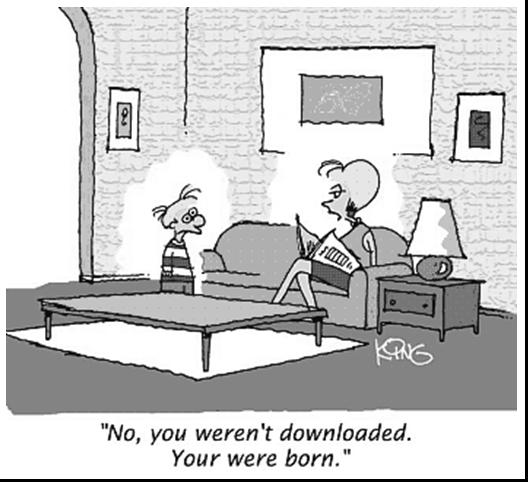
\includegraphics[width=.5\textwidth]{fig1.jpg}
\caption{A typical figure}
\label{fig:exampleFig1}
\end{figure}

\begin{figure}[ht]
\centering
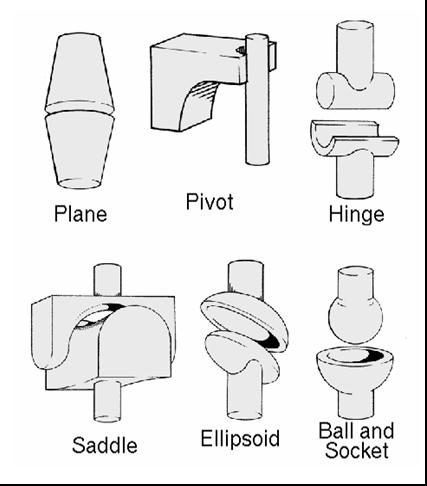
\includegraphics[width=.3\textwidth]{fig2.jpg}
\caption{This figure is an example of a figure caption taking more than one
  line and justified considering margins mentioned in Section~\ref{sec:figs}.}
\label{fig:exampleFig2}
\end{figure}

In tables, try to avoid the use of colored or shaded backgrounds, and avoid
thick, doubled, or unnecessary framing lines. When reporting empirical data,
do not use more decimal digits than warranted by their precision and
reproducibility. Table caption must be placed before the table (see Table 1)
and the font used must also be Helvetica, 10 point, boldface, with 6 points of
space before and after each caption.



\begin{thebibliography}{99}

\bibitem{SousaFilho2012} FILHO, G. S. et al. Uma arquitetura e ferramentas para problemas de localização de facilidades no setor público. São Paulo: SBC, 2012. Disponível em: <https://sol.sbc.org.br/index.php/sbsi/article/view/14428>

\bibitem{KuoKung2025} KUNG, L.-C.; CHUANG, J.-S.; KUO, Y.-T. Optimal Allocation of Capacitated Facilities considering Time-dependent User Preference for User Number Maximization. Disponível em: <https://ssrn.com/abstract=4276750>. Acesso em: 5 set. 2025. 

\bibitem{Buesing2025} BÜSING, C.; GERSING, T.; WREDE, S. Insights into the computational complexity of the single-source capacitated facility location problem with customer preferences. [s.l.] Optimization Online, dez. 2024. 

\bibitem{Kang2023} KANG, C.-N. et al. A service facility location problem considering customer preference and facility capacity. Computers \& Industrial Engineering, v. 177, p. 109070, 2023.

\bibitem{OwenDaskin1998} OWEN, S. H.; DASKIN, M. S. Strategic facility location: A review. European Journal of Operational Research, v. 111, p. 423–447, 1998. 

\end{thebibliography}

\end{document}